%\chapter{開発プロセス}
\section{第1サイクル}
第1サイクルはプロジェクト発足から中間発表会用のポスターレビューまでとした。本サイクルでは第1回フィールドワークからの経験から、木古内町の観光情報が分散していること、観光中に撮影した写真が整理されていないことを問題として定義した。最初の設計段階であがった案は以下の5つであり具体的な画面イメージを作成できたのはマップ画面、Webページを表示する画面、お散歩コースを表示する画面の3つである。これらの案に対するレビューを6月12日に行った外部講師とのテレビ会議で受けた結果、現在の提案に木古内らしさを加える必要があるとの指摘を受けた。
\begin{itemize}
 \item マップ上に表示されたピンをタップすると吹き出しとして詳細情報をクイック表示する機能
 \item 吹き出しをタップするとお店のWebページへ画面遷移する機能
 \item 木古内町民しか知らないニュースや、木古内町の天気をマップ画面に表示する
 \item ユーザ同士で木古内町の写真を共有できる機能
 \item 木古内観光協会が公開している木古内お散歩コースをマップの中に盛り込む
\end{itemize}

\begin{figure}[htbp]
  \begin{center}
    \begin{tabular}{c}

      % 1
      \begin{minipage}{0.33\hsize}
        \begin{center}
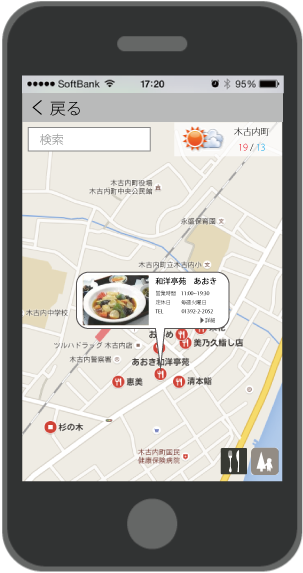
\includegraphics[width=4cm, bb=0 0 303 573]{5.2_map1.png}
          \hspace{1cm} (a)観光スポットの紹介
        \end{center}
      \end{minipage}

      % 2
      \begin{minipage}{0.33\hsize}
        \begin{center}
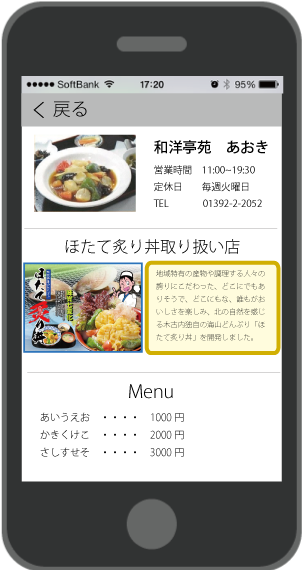
\includegraphics[width=4cm, bb=0 0 304 570]{5.2_map2.png}
          \hspace{1cm} (b)観光スポットの詳細情報
        \end{center}
      \end{minipage}

      % 3
      \begin{minipage}{0.33\hsize}
        \begin{center}
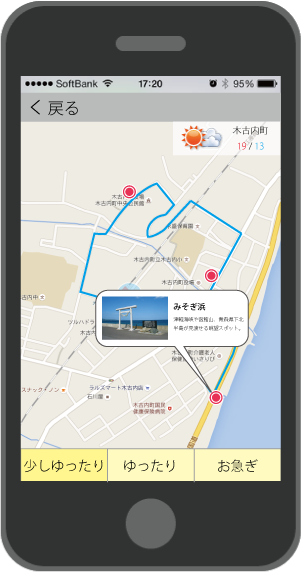
\includegraphics[width=4cm, bb=0 0 302 572]{5.2_sanpo.png}
          \hspace{1cm} (c)お散歩コース
        \end{center}
      \end{minipage}

    \end{tabular}
    \caption{初期段階での画面イメージ}
    \label{fig:lena}
  \end{center}
\end{figure}

その後は上記5つの案に対して議論を行い、木古内町民しか知らないニュースは継続運用が困難であるという理由から実装を保留した。また、木古内観光協会が公開している木古内お散歩コースをマップの中に盛り込む機能は公開されていたコース内容が車での移動を前提にしており、自分たちでコースを作らなければいけないという理由から実装は保留となった。この段階で実装した機能は以下の3つである。しかし、中間発表会用のポスターレビューの際にユーザストーリに問題があるとの指摘を受けた。具体的には、観光客は観光スポットやランドマークの写真を見てからその場所へ行くのが通常の流れである。しかし、当時作成していたアプリは場所を伝えてから写真や詳細情報を見せる流れになってしまっていた。この状態だと木古内町の魅力はもちろんのこと、何があるかすら伝わらないとの内容であった。この指摘を受けて先に伝える情報は場所ではなく内容にすべきという結論に達した。そして中間発表会までに改善することをメンバー間で合意し、第2サイクルへ移行した。
\begin{itemize}
 \item マップ上に表示されたピンをタップすると吹き出しとして詳細情報をクイック表示する機能
 \item 木古内町の天気を表示する
 \item 現在地から目的地までのルート案内
\end{itemize}

\addtocounter{figure}{-1}
\begin{figure}[htbp]
  \begin{center}
    \begin{tabular}{c}

      % 1
      \begin{minipage}{0.33\hsize}
        \begin{center}
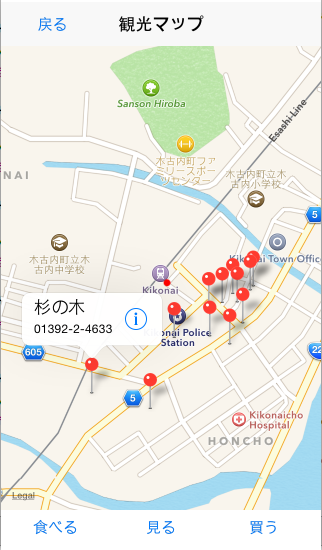
\includegraphics[width=4cm, bb=0 0 322 550]{5.3_map1.png}
          \hspace{1cm} (d)詳細情報のクイック表示
        \end{center}
      \end{minipage}

      % 2
      \begin{minipage}{0.33\hsize}
        \begin{center}
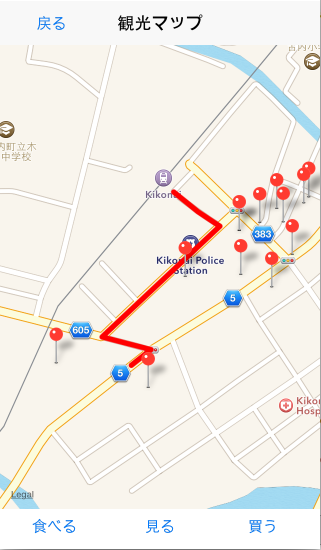
\includegraphics[width=4cm, bb=0 0 321 550]{5.3_map2.png}
          \hspace{1cm} (e)ルート案内
        \end{center}
      \end{minipage}

      % 3
      \begin{minipage}{0.33\hsize}
        \begin{center}
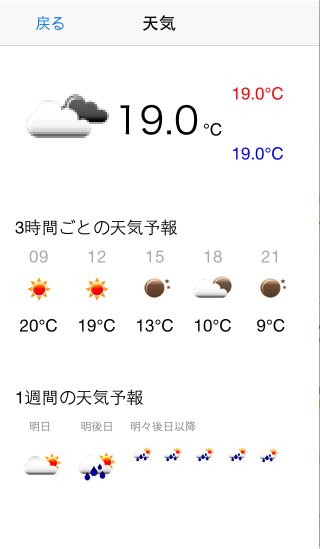
\includegraphics[width=4cm, bb=0 0 320 549]{5.3_weather.png}
          \hspace{1cm} (f)木古内町の天気を表示
        \end{center}
      \end{minipage}

    \end{tabular}
    \caption{第1サイクルでの完成画面 }
    
    \label{fig:lena}
  \end{center}
\end{figure}
\bunseki{岩見建汰}